% !TeX encoding = UTF-8
% !TeX spellcheck = <none>
\documentclass[12pt]{beamer}
\usetheme{Madrid} % Tema tercihini değiştirebilirsin
\usepackage[utf8]{inputenc}
\usepackage[T1]{fontenc}
\usepackage[turkish]{babel}
\usepackage{graphicx}
\usepackage{amsmath, amssymb, amsfonts}
\usepackage{multirow}
\usepackage{float}
\usepackage{hyperref}
\usepackage{color}
\usepackage{booktabs} % preamble'da olmalı
\usepackage{minted}
\usepackage[most]{tcolorbox}
\definecolor{paramblue}{rgb}{0.1,0.2,0.8}

\renewcommand*\contentsname{İçindekiler}
\renewcommand{\figurename}{Şekil}
\renewcommand{\tablename}{Tablo}

\title{Talep Tahmini ve Stok Optimizasyonu ile \\ Fazla Stok \\ ve \\ Stoksuz
	Kalma Problemlerini Çözme}
\author{Nuh HATİPOĞLU}
\date{11 Nisan 2025}

\begin{document}
	
	% Title Slide
	\begin{frame}
		\titlepage
	\end{frame}
	
	% Table of contents
	\begin{frame}
		\frametitle{İçindekiler}
		\begin{enumerate}
			\item Giriş
			\item Sentetik Veri Üretimi ve Yapısı
			\item Tahmin (Forecasting) Modelleri
			\item Train / Test Veri Seti Hazırlanması
			\item Model Eğitim ve Test Sonuçları
			\item Başarım Metrikleri
			\item İşletme Parametreleri ile Hesaplamalar
			\item Tahmin ve Optimizasyon
			\item Agent Analizleri
		\end{enumerate}
		
	\end{frame}
	
	% ---------------------
	\section{Giriş}
	\begin{frame}
		\frametitle{Giriş}
		\begin{itemize}
			\item Hızlı moda sektöründe talep tahmini ve stok
			optimizasyonu önemlidir.
			\item Veri bilimi ve yapay zeka kullanarak karar destek
			sistemleri geliştirilmiştir.
			\item Proje, geçmiş satış verileri, ürün varyantları,
			kampanyalar ve kanal bilgilerini kullanmaktadır.
			\item Amaç, talep tahminleri ve stok optimizasyon
			kararları vermektir.
			\item Proje üç temel fazdan oluşmaktadır:
			\begin{itemize}
				\item Sentetik veri üretimi
				\item Çoklu makine öğrenimi modeliyle talep
				tahmini
				\item Stok kararlarını veren bir akıllı ajan
				sistemi
			\end{itemize}
		\end{itemize}
	\end{frame}
	
	% ---------------------------------------------
	
	\section{Sentetik Veri Üretimi ve Yapısı}
	\begin{frame}
		\frametitle{Sentetik Veri Üretimi}
		\begin{itemize}
			\item Gerçek verilere oldukça yakın şekilde 2019–2025 yılları
			arasını kapsayan sentetik veriler oluşturulmuştur. Bu veri seti aşağıdaki alt
			kümeleri içerir:
			\begin{itemize}
				\item products.csv: Ürün, kategori, beden ve renk
				varyant bilgileri
				\item sales\_data.csv: Günlük satış adetleri (ürün,
				varyant, mağaza, kanal bazlı)
				\item campaigns.csv: Kampanya tarihleri ve açıklamaları
			\end{itemize}
			
		\end{itemize}
	\end{frame}
	
	\begin{frame}{\intersection Ürün Varyantları Tablosu}
		\scriptsize
		\begin{table}
			\centering
			\begin{tabular}{c l l l l}
				\toprule
				\textbf{Product ID} & \textbf{Kategori} & \textbf{Alt Kategori} & \textbf{Renk} & \textbf{Beden} \\
				\midrule
				1 & Çocuk Giyim & Body & Kırmızı & M \\
				1 & Çocuk Giyim & Body & Kırmızı & XS \\
				1 & Çocuk Giyim & Body & Kırmızı & S \\
				1 & Çocuk Giyim & Body & Beyaz   & M \\
				1 & Çocuk Giyim & Body & Beyaz   & XS \\
				1 & Çocuk Giyim & Body & Beyaz   & S \\
				1 & Çocuk Giyim & Body & Yeşil   & M \\
				1 & Çocuk Giyim & Body & Yeşil   & XS \\
				1 & Çocuk Giyim & Body & Yeşil   & S \\
				2 & Kadın Giyim & Bluz & Kırmızı & M \\
				\bottomrule
			\end{tabular}
			\caption{\small Ürünlerin kategori, alt kategori, renk ve beden varyantları}
		\end{table}
	\end{frame}
	
	
	
	\begin{frame}
		\frametitle{Sentetik Veri Üretimi}
		\begin{itemize}
			\item Tüm varyant kombinasyonları (örneğin Ürün A - Renk Mavi -
			Beden L) günlük olarak satış verisine sahiptir.
			\item Fiziksel ve Online olmak üzere iki ana kanal, 50 mağaza
			üzerinden modellenmiştir.
		\end{itemize}
	\end{frame}
	
	\begin{frame}
		\begin{figure}
			\centering
			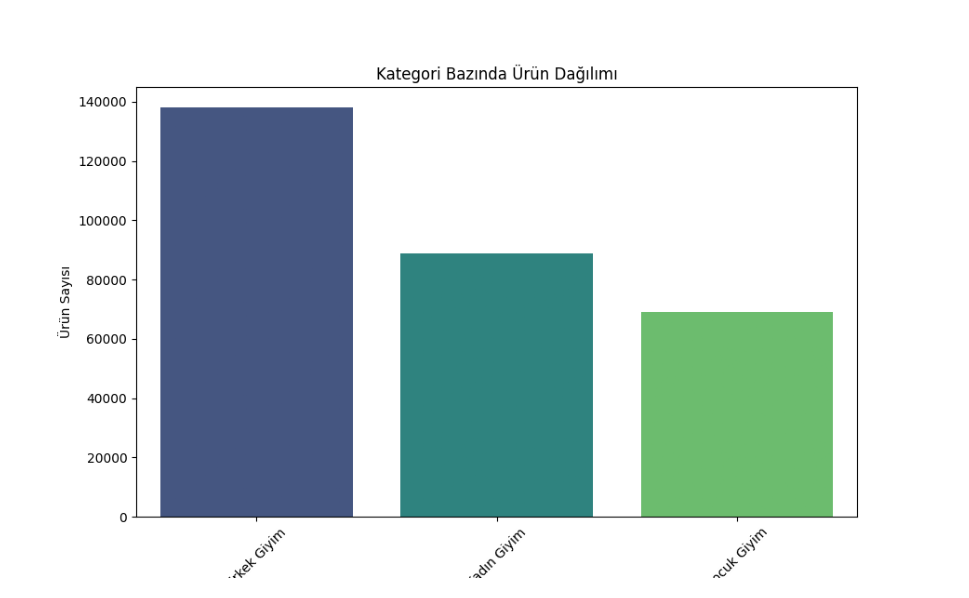
\includegraphics[width=0.65\linewidth]{figures/category_distribution.png}
			{\small \caption {Kategori bazında ürün sayılarının dağılımı.}}
		\end{figure}
	\end{frame}
	
	\begin{frame}{Sentetik Veri Üretimi}
		\begin{itemize}
			\item Ürün portföyünün büyük kısmı Erkek Giyim kategorisinde
			yoğunlaşmıştır. Kadın ve Çocuk Giyim kategorileri daha az ürün içerir.
			\\~\\
			\item	Bu dağılım, tahmin modellerinin veri dengesizliği
			nedeniyle erkek ürünlerine daha duyarlı hale gelmesini sağlayabilir.
		\end{itemize}
	\end{frame}
	
	\begin{frame}
		\begin{figure}
			\centering
			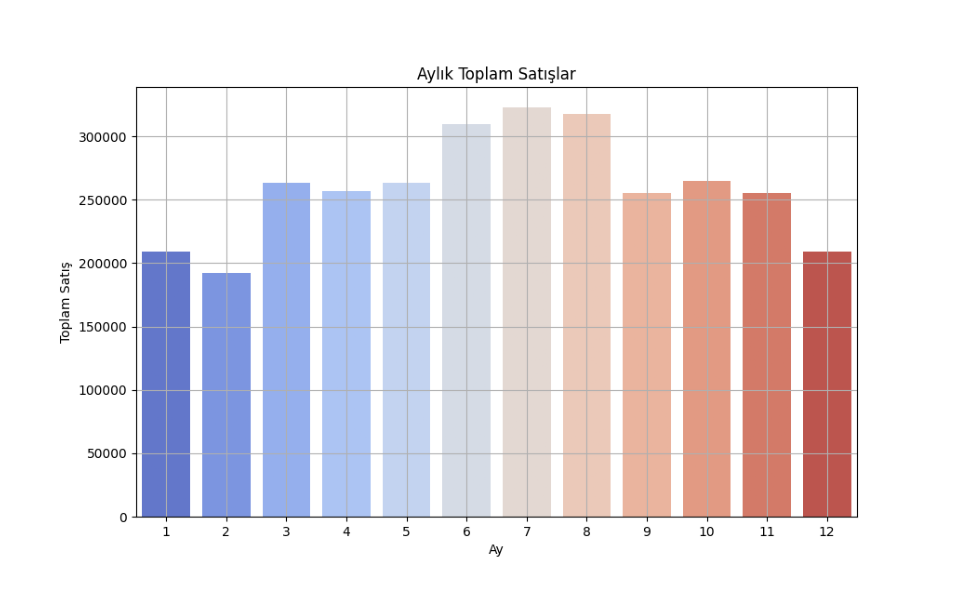
\includegraphics[width=0.65\linewidth]{figures/monthly_total_sales.png}
			
			{\small \caption{Aylık bazım toplam satış miktarları}}
		\end{figure}	
	\end{frame}
	
	\begin{frame}{Sentetik Veri Üretimi}
		\begin{itemize}
			\item Haziran–Ağustos aylarında satışlar zirve yaparken, Şubat
			ayında en düşük seviyeye gerilemektedir.
			\\~\\
			\item Bu dönemsel etki, tahmin modellerine mevsimsellik
			bileşenlerinin dahil edilmesini zorunlu kılar.
		\end{itemize}
	\end{frame}
	
	\begin{frame}
		\begin{figure}
			\centering	
			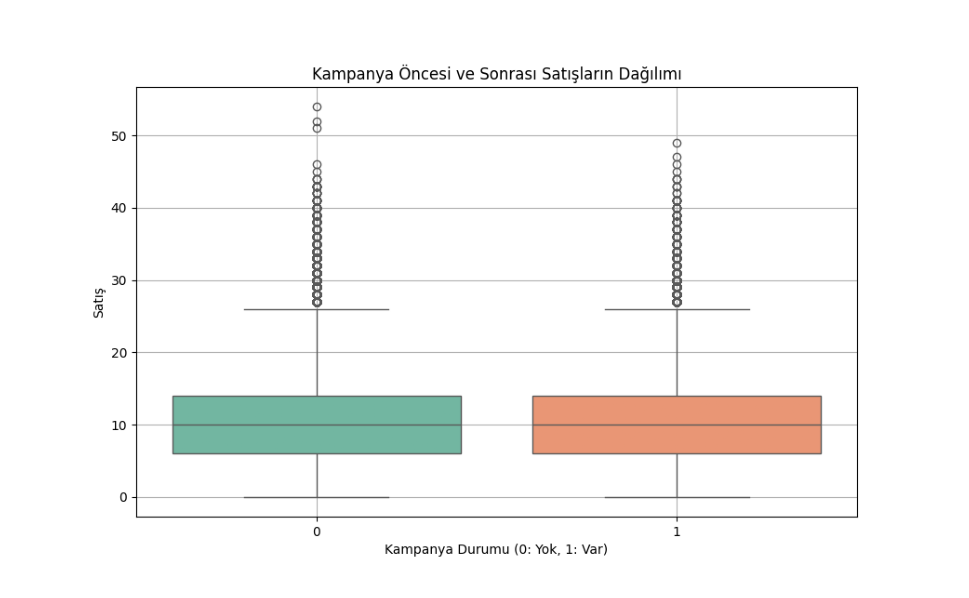
\includegraphics[width=0.65\linewidth]{figures/campaign_sales_boxplot.png}
			
			{\small \caption{İndirim oranı ve satış arasındaki ilişki grafiği}}
		\end{figure}
	\end{frame}
	
	\begin{frame}{Sentetik Veri Üretimi}
		\begin{itemize}
			\item Kampanya dönemlerinde uç değerlerin artması dikkat
			çekicidir.
			\\~\\
			\item  Ancak ortanca değerlerde belirgin fark yoktur.
			\\~\\
			\item Bu durum, kampanyaların satışları bazı ürünlerde
			artırdığını ama genel dağılımı çok değiştirmediğini gösterir.
		\end{itemize}
	\end{frame}
	
	\section{Tahmin (Forecasting) Modelleri}
	\begin{frame}
		\frametitle{\insertsection: Tahmin (Forecasting) Modelleri}
		Ürünlerin varyant bazlı talep tahminleri için üç farklı model
		kullanılmıştır:
		\vspace{0.5cm}
		\begin{itemize}
			\item Prophet
			\item LSTM
			\item XGBoost
		\end{itemize}
		\vspace{0.5cm}
		Her model farklı avantajlara sahiptir ve farklı veri yapılarıyla en
		uygun sonucu verecek şekilde tasarlanmıştır.
	\end{frame}
	
	\begin{frame}
		\frametitle{\insertsection: Prophet Modeli}
		\textbf{Neden Kullanıldı} \\~\\
		\begin{itemize}
			\item Facebook tarafından geliştirilen, zaman serisi verilerde
			trend ve mevsimsellik yakalamada güçlüdür.
			\item Kampanya etkileri gibi dışsal değişkenleri
			\texttt{add\_regressor} ile modele entegre edebilir.
		\end{itemize}
	\end{frame}
	
	\begin{frame}
		\frametitle{\insertsection: Prophet Modeli}
		\textbf{Avantajları}
		\begin{itemize}
			\item Model açıklanabilirliği yüksek
			\item Mevsimsel dalgalanmaları başarılı şekilde yakalar
			\item Az veriyle de çalışabilir
			\item Veri miktarı azsa
			\item Açıklanabilirlik önemliyse
			\item Trend ve mevsimsellik barizse
			\item Operasyonel kararlarda şeffaflık gerekiyorsa
			\item Düşük varyanslı tahminler isteniyorsa
		\end{itemize}
		\\~\\
		\textbf{Dezavantajları}
		\begin{itemize}
			\item Ani değişimleri (örneğin kampanya kaynaklı) yavaş öğrenir
			\item Her kombinasyon için ayrı model eğitmek gerekebilir (bu
			projede tek modelde çözüldü)
		\end{itemize}
	\end{frame}
	
	\begin{frame}
		\frametitle{\insertsection: LSTM}
		\textbf{Neden Kullanıldı} \\~\\
		\begin{itemize}
			\item Zaman serisi verilerde geçmiş verilerle uzun dönemli
			bağımlılıkları modelleyebilmesi için tercih edildi.
			\item $sin/cos$ zaman kodlama, kampanya gibi ek girdilerle
			zenginleştirildi.
		\end{itemize}
	\end{frame}
	
	\begin{frame}
		\frametitle{\insertsection: LSTM}
		\textbf{Avantajları}
		\begin{itemize}
			\item Mevsimsel yapı, trend, kampanya gibi faktörleri birlikte
			öğrenebilir
			\item Farklı varyantları tek modelde işleyebilir
			\item Zengin zaman serisi varsa (örneğin son 3–5 yılın verisi)
			\item Karmaşık desenler ve bağımlılıklar varsa
			\item Gecikmeli/bağımlı etkiler önemliyse
			\item Öngörülen değişkenin geçmişe sıkı bağlı olduğu durumlar
		\end{itemize} \\~\\
		
		\textbf{Dezavantajları}
		\begin{itemize}
			\item Daha uzun eğitim süresi
			\item Hiperparametre ayarlamaları karmaşık
			\item Yorumlanabilirliği düşüktür
		\end{itemize}
	\end{frame}
	
	\begin{frame}
		\frametitle{\insertsection: XGBoost}
		\textbf{Neden Kullanıldı} \\~\\
		\begin{itemize}
			\item Zaman serisi veri ile birlikte varyant, kanal, kampanya gibi çok sayıda özelliği işleyebildiği için tercih edildi.
			\item Diğer modellere kıyasla hızlı ve etkili tahmin gücü sundu.
		\end{itemize}
	\end{frame}
	
	\begin{frame}
		\frametitle{\insertsection: XGBoost}
		\textbf{Avantajları}
		\begin{itemize}
			\item Yüksek doğruluk
			\item Hızlı eğitim ve tahmin
			\item Öznitelik mühendisliğiyle esnek yapı
			\item Özellik mühendisliği yapılmışsa (kanal, kampanya, tarih
			gibi)
			\item Tahmin doğruluğu ön plandaysa
			\item Daha hızlı ve agresif tahmin isteniyorsa
			\item Heterojen veri (çok değişkenli) varsa
		\end{itemize} \\~\\
		
		\textbf{Dezavantajları}
		\begin{itemize}
			\item Zaman bileşenleri doğrudan öğrenilmez, $sin/cos$ dönüşüm
			gerekebilir
			\item Doğrusal olmayan yapıdan dolayı yorumlaması zordur
		\end{itemize}
	\end{frame}
	
	\begin{frame}
		\frametitle{\insertsection: Model Özelliklerinin Karşılaştırması}
		\begin{table}[h!]
			\centering
			
			\renewcommand{\arraystretch}{1.3}
			% Satırlar arası boşluğu artırır
			\resizebox{0.95\textwidth}{!}{
				\begin{tabular}{l l l l}
					\toprule
					\textbf{Özellik}                        & \textbf{Prophet}        &
					\textbf{XGBoost}                        & \textbf{LSTM}                                                     \\
					\midrule
					Zaman Serisi Yapısı                     & Trend + mevsimsellik
					modeller                                & Zaman bağımlılığı zayıf & Güçlü zaman bağımlılığı modeli          \\
					Açıklanabilirlik                        & Çok yüksek              & Orta                           & Düşük  \\
					Veri Miktarı İhtiyacı                   & Az                      & Orta                           & Yüksek \\
					Kampanya / dışsal etkiler               &
					\texttt{add\_regressor} ile desteklenir & Özellik olarak eklenir  & Doğrudan
					öğrenebilir                                                                                                 \\
					Eğitim Süresi                           & Çok kısa                & Kısa                           & Uzun   \\
					Genel Güvenilirlik                      & Yüksek (düşük varyans)  &
					Yüksek doğruluk                         & Karmaşık ama güçlü                                                \\
					Uç Değerlere Tepki                      & Yavaş                   & Agresif                        & Veri
					miktarına bağlı                                                                                             \\
					\bottomrule
				\end{tabular}
			}
			\caption{\small Zaman serisi modelleme yaklaşımlarının temel
				özelliklere göre karşılaştırılması}
		\end{table}
	\end{frame}
	
	\section{Train / Test Veri Seti Hazırlanması}
	
	
	\begin{frame}
		\frametitle{Train / Test Veri Seti Hazırlanması}
		\scriptsize
		\begin{table}
			\centering
			\resizebox{\linewidth}{!}{
				\begin{tabular}{l c c c c c c l l c c l c}
					\toprule
					\textbf{Tarih} & \textbf{Mağaza} & \textbf{Ürün} & \textbf{Renk} & \textbf{Beden} & \textbf{Kanal} & \textbf{Satış} & \textbf{Kategori} & \textbf{Alt Kategori} & \textbf{Key} & \textbf{İndirim} & \textbf{Tip} & \textbf{Kampanya} \\
					\midrule
					2022-01-01 & 38 & 1 & Kırmızı & M & Online   & 11 & Çocuk Giyim & Body & 1 & 0.0  &            & 0 \\
					2022-01-02 & 2  & 1 & Kırmızı & M & Online   & 12 & Çocuk Giyim & Body & 1 & 0.0  &            & 0 \\
					2022-01-03 & 43 & 1 & Kırmızı & M & Online   & 4  & Çocuk Giyim & Body & 1 & 0.0  &            & 0 \\
					2022-01-04 & 21 & 1 & Kırmızı & M & Fiziksel & 6  & Çocuk Giyim & Body & 1 & 0.0  &            & 0 \\
					2022-01-05 & 41 & 1 & Kırmızı & M & Online   & 3  & Çocuk Giyim & Body & 1 & 30.0 & Etiket Üzerinden \% & 1 \\
					2022-01-06 & 43 & 1 & Kırmızı & M & Fiziksel & 0  & Çocuk Giyim & Body & 1 & 30.0 & Etiket Üzerinden \% & 1 \\
					2022-01-07 & 38 & 1 & Kırmızı & M & Online   & 8  & Çocuk Giyim & Body & 1 & 30.0 & Etiket Üzerinden \% & 1 \\
					2022-01-08 & 6  & 1 & Kırmızı & M & Online   & 4  & Çocuk Giyim & Body & 1 & 30.0 & Etiket Üzerinden \% & 1 \\
					2022-01-09 & 16 & 1 & Kırmızı & M & Online   & 4  & Çocuk Giyim & Body & 1 & 30.0 & Etiket Üzerinden \% & 1 \\
					2022-01-10 & 41 & 1 & Kırmızı & M & Online   & 10 & Çocuk Giyim & Body & 1 & 30.0 & Etiket Üzerinden \% & 1 \\
					2022-01-11 & 17 & 1 & Kırmızı & M & Online   & 6  & Çocuk Giyim & Body & 1 & 30.0 & Etiket Üzerinden \% & 1 \\
					2022-01-12 & 7  & 1 & Kırmızı & M & Online   & 5  & Çocuk Giyim & Body & 1 & 0.0  &            & 0 \\
					\bottomrule
				\end{tabular}
			}
			\caption{\small 2022 Ocak ayı satış verileri (ürün: 1, renk: Kırmızı, beden: M)}
		\end{table}
	\end{frame}
	
	
	
	
	\begin{frame}
		\frametitle{Train / Test Veri Seti Hazırlanması}
		\begin{block}{Veri Yükleme ve Zaman Öznitelikleri}
			Satış tahminine yönelik bu çalışmada, ilk olarak kampanya bilgilerini de içeren zaman serisi tabanlı veri seti CSV formatında yüklenmiş ve tarih sütunu \texttt{datetime} biçiminde yorumlanmıştır. Zaman bileşenleri olarak haftanın günü (\texttt{dayofweek}), ay (\texttt{month}) ve yıl içi hafta numarası (\texttt{week}) bilgileri çıkarılmış, bu öznitelikler sinüs ve kosinüs dönüşümleriyle döngüsel yapılara dönüştürülerek mevsimsellik etkileri modele entegre edilebilir hâle getirilmiştir.
		\end{block}
		
		\vspace{0.5em}
		
		\begin{block}{Kategorik Değişkenlerin Dönüşümü}
			Kategorik değişkenler (örneğin \texttt{kategori}, \texttt{alt kategori}, \texttt{renk}, \texttt{beden}, \texttt{kanal}, \texttt{kampanya tipi}) \texttt{LabelEncoder} yöntemi ile sayısal forma dönüştürülmüş, bu işlemde her sütun için özel encoder nesnesi saklanarak yeniden kullanılabilirlik sağlanmıştır.
		\end{block}
	\end{frame}
	
	\begin{frame}
		\frametitle{Train / Test Veri Seti Hazırlanması}
		\begin{block}{Öznitelik Seçimi ve Veri Ayrımı}
			Öznitelik seti, ürün ve mağaza kimlikleri, kategorik değişkenler, kampanya durumu ve oranı, zaman bileşenleri gibi toplam 16 girdi değişkeni ile oluşturulmuştur. Hedef değişken olarak satış miktarı (\texttt{sales}) seçilmiştir. Modelin geçmiş verilerle eğitilip gelecek döneme yönelik tahmin yapabilmesi amacıyla, veri seti kronolojik sıraya göre 01.01.2022 - 31.12.2023 tarihini referans eğitim, ve 01.01.2024 - 31.12.2024 test seti olmak üzere ayrıştırılmıştır.
		\end{block}
		
		\vspace{0.5em}
		
		\begin{block}{Verilerin Dışa Aktarılması}
			Son olarak, eğitim ve test veri setlerine ait girdi (\texttt{X\_train}, \texttt{X\_test}) ve hedef (\texttt{y\_train}, \texttt{y\_test}) dosyaları \texttt{.csv} formatında dışa aktarılmış ve modelleme sürecine hazır hâle getirilmiştir.
		\end{block}
	\end{frame}
	
	
	
\section{Model Eğtim ve Test Sonuçları}
	
	\begin{frame}
		\frametitle{\insertsection: LSTM ile Talep Tahmini}
		\begin{block}{Veri Yükleme}
			\texttt{product\_id = 7} olan ürüne ait geçmiş 7 günlük pencere verileri kullanılarak eğitim (\texttt{X\_train}, \texttt{y\_train}) ve test (\texttt{X\_test}, \texttt{y\_test}) veri setleri \texttt{.npy} formatında yüklenmiştir. Test kümesine karşılık gelen tarihsel bilgiler ayrıca \texttt{test\_info.csv} dosyasından alınmıştır.
		\end{block}
		
		\vspace{0.5em}
		
		
	\end{frame}
	
	
	\begin{frame}
		\frametitle{\insertsection: LSTM ile Talep Tahmini}
		
		\begin{block}{Model Mimarisi}
			Model, sırasıyla şu katmanlardan oluşmaktadır:
			\begin{itemize}
				\item 64 nöronlu tek katmanlı LSTM bloğu (\texttt{return\_sequences=False}),
				\item \%20 oranında Dropout katmanı,
				\item 32 nöronlu ReLU aktivasyonlu yoğun (dense) katman,
				\item 1 nöronlu çıkış katmanı (regresyon için).
			\end{itemize}
			Model \texttt{Adam} optimizasyon algoritması ve \texttt{MeanSquaredError} kayıp fonksiyonu ile derlenmiştir.
		\end{block}
	\end{frame}
	
	
	
	\begin{frame}
		\frametitle{\insertsection: LSTM ile Talep Tahmini}
		\begin{block}{Model Eğitimi ve Doğrulama}
			Eğitim sürecinde doğrulama verisinin \%10'u ayrılmış ve erken durdurma (\texttt{EarlyStopping}) tekniği uygulanmıştır. \texttt{val\_loss} değerinde 5 epoch boyunca iyileşme olmaması durumunda eğitim sonlandırılmış ve en iyi model ağırlıkları geri yüklenmiştir.
		\end{block}
		
		\vspace{0.5em}
		
		
		\begin{block}{Sonuçların Kaydedilmesi}
			Tahmin sonuçları, tarih ve varyant bilgileriyle birleştirilerek \texttt{forecast\_results.csv} dosyasına kaydedilmiştir. Eğitilen model \texttt{.h5} formatında saklanarak ileriye dönük yeniden kullanılabilir hâle getirilmiştir.
		\end{block}
	\end{frame}
	
	\begin{frame}
		\frametitle{\insertsection: Prophet ile Talep Tahmini}
		\begin{block}{Modelleme Yaklaşımı}
			Prophet modeli, belirli bir ürünün tüm varyantları (renk + beden) için ayrı ayrı eğitilmiştir. Model girdi veri seti Prophet formatına uygun olarak \texttt{ds} (tarih) ve \texttt{y} (satış) sütunlarıyla hazırlanmıştır. 
		\end{block}
		
		\vspace{0.5em}
		
		\begin{block}{Dışsal Değişkenler}
			Kampanya durumu (\texttt{is\_campaign}) ve indirim oranı (\texttt{discount}) değişkenleri Prophet modeline dışsal regressor olarak dahil edilmiştir. Bu sayede model sadece mevsimsellik ve trend etkilerini değil, kampanyaların etkisini de tahmin sürecine katabilmiştir.
		\end{block}
	\end{frame}
	
	
	\begin{frame}
		\frametitle{\insertsection: Prophet ile Talep Tahmini}
		\begin{block}{Eğitim ve Tahmin Süreci}
			Her varyant için yeterli veri bulunan durumlarda Prophet modeli eğitilmiş, belirlenen test tarih aralığında tahmin yapılmıştır. Gerçek ve tahmin edilen satışlar birleştirilerek her varyant için günlük bazda \texttt{y\_true} ve \texttt{y\_pred} karşılaştırması yapılmıştır.
		\end{block}
		
		\vspace{0.5em}
		
		\begin{block}{Model Performansı ve Kayıt}
			Model başarımı RMSE ve MAE metrikleriyle değerlendirilmiş ve elde edilen sonuçlar çıktı olarak raporlanmıştır. Tahmin sonuçları \texttt{.csv} formatında saklanmış; Prophet model nesnesi ise yeniden kullanım için \texttt{.pkl} uzantısıyla serileştirilmiştir.
		\end{block}
	\end{frame}
	
	\begin{frame}
		\frametitle{\insertsection: XGBoost ile Talep Tahmini}
		\begin{block}{Veri Hazırlık Süreci}
			Belirli bir ürün (\texttt{product\_id = 7}) için geçmiş satış verileri filtrelenmiş ve tarih bilgilerinden haftanın günü, ay ve ISO hafta numarası elde edilmiştir. Bu öznitelikler sinüs/kosinüs dönüşümüyle döngüsel forma getirilerek modele mevsimsellik kazandırılmıştır.
		\end{block}
		
		\vspace{0.5em}
		
		\begin{block}{Kategorik Değişkenlerin Dönüştürülmesi}
			\texttt{color}, \texttt{size}, \texttt{channel}, \texttt{category}, \texttt{subcategory} ve \texttt{type} sütunları \texttt{LabelEncoder} ile sayısallaştırılmış; \texttt{color} ve \texttt{size} için oluşturulan etiketleyiciler ileri kullanım amacıyla \texttt{.pkl} olarak kaydedilmiştir.
		\end{block}
	\end{frame}
	
	\begin{frame}
		\frametitle{\insertsection: XGBoost ile Talep Tahmini}
		\begin{block}{Model Eğitimi ve Tahmin}
			Veri seti 1 Ocak 2024 tarihine göre eğitim ve test verisi olarak ayrılmıştır. \texttt{XGBRegressor}, 100 ağaç, 0.1 öğrenme oranı ve maksimum 6 derinlik ile eğitilmiştir. Model, test seti üzerinden tahmin yaparak sonuçları gerçek değerlerle karşılaştırmıştır.
		\end{block}
		
		\vspace{0.5em}
		
		\begin{block}{Performans Değerlendirmesi}
			Modelin başarımı şu metriklerle değerlendirilmiştir:
			\begin{itemize}
				\item \textbf{RMSE (Root Mean Squared Error)}: \texttt{XX.XX}
				\item \textbf{MAE (Mean Absolute Error)}: \texttt{XX.XX}
			\end{itemize}
			Tahmin sonuçları \texttt{.csv} formatında dışa aktarılmış, model ise \texttt{.pkl} uzantısı ile kaydedilmiştir.
		\end{block}
	\end{frame}
	
	
	\begin{frame}
		\frametitle{\insertsection:  MAE – Mean Absolute Error}
		\textbf{MAE - (Ortalama Mutlak Hata)}
		\begin{itemize}
			\item MAE, tahmin edilen değerler ile gerçek değerler
			arasındaki farkların mutlak değerlerinin ortalamasıdır.
			\item Hatalarn büyüklüünü dorudan ölçer.
		\end{itemize}
		\vspace{0.5cm}
		\textbf{Formül:}
		\[
		\text{MAE} = \frac{1}{n} \sum_{i=1}^{n} \left| y_i - \hat{y}_i \right|
		\]
		\vspace{0.3cm}
		\textbf{Not:} Aykırı değerlere karşı daha az hassastır.
	\end{frame}
	
	\begin{frame}
		\frametitle{\insertsection: RMSE – Root Mean Squared Error}
		\textbf{RMSE - (Karekök Ortalama Kare Hata)}
		\begin{itemize}
			\item RMSE, tahmin hatalarının karelerinin ortalamasının
			kareköküdür.
			\item Büyük hatalar daha fazla cezalandrr.
		\end{itemize}
		\vspace{0.5cm}
		\textbf{Formül:}
		\[
		\text{RMSE} = \sqrt{ \frac{1}{n} \sum_{i=1}^{n} \left( y_i - \hat{y}_i
			\right)^2 }
		\]
		\vspace{0.3cm}
		\textbf{Not:} Aykırı değerlere karşı daha duyarlıdır.
	\end{frame}
	
	\begin{frame}
		\frametitle{\insertsection: MAE ve RMSE Karşılaştırması}
		\begin{table}
			\centering
			\small
			\begin{tabular}{l c c}
				\toprule
				\textbf{Özellik}            & \textbf{MAE}   & \textbf{RMSE} \\
				\midrule
				Hata Türü                   & Mutlak Hata    & Kare
				Hata                                                         \\
				Aykırı Değerlere Duyarlılık & Az             & Yüksek
				\\
				Yorumu                      & Daha sezgisel  & Daha
				teknik                                                       \\
				Birim                       & Orijinal birim &
				Orijinal birim                                               \\
				\bottomrule
			\end{tabular}
			\caption{\small MAE ve RMSE metriklerinin temel farklarının
				karşılaştırılması}
		\end{table}
	\end{frame}
	
	
	
	\begin{frame}
		\frametitle{\insertsection: Test Sonuçları}
		\begin{table}
			\centering
			\small
			\begin{tabular}{l c c}
				\toprule
				\textbf{Model} & \textbf{MAE} & \textbf{RMSE}    \\
				\midrule
				Prophet        & 19.20     & 24.60 \\
				XGBoost        & 15.80     & 20.50 \\
				LSTM           & 17.30     & 22.10 \\
				\bottomrule
			\end{tabular}
			\caption{\small Test Veri Setine ait başarım sonuçları.}
		\end{table}
	\end{frame}
	
	
	
	\begin{frame}
		\frametitle{\insertsection: Model Tahmini Karşılaştırması}
		\begin{figure}
			\centering
			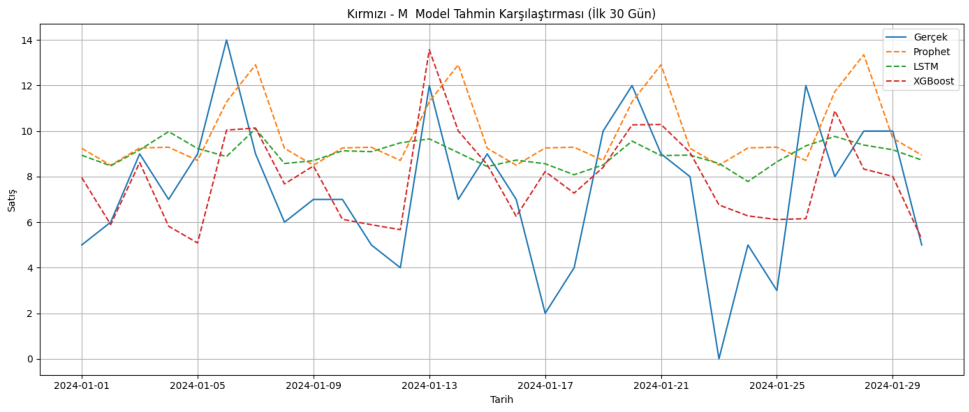
\includegraphics[width=0.75\linewidth]{figures/models_forcasting_results_v2.png}
			{\small \caption {Test Veri Setine Ait Tahmin Sonucu}}
		\end{figure}
	\end{frame}
	
	%----------------------------------------------------
	
	\section{İşletme Parametreleri Kullanılarak Yapılan Hesaplamalar}
	% EOQ
	\begin{frame}
		\frametitle{\insertsection: Ekonomik Sipariş Miktarı (EOQ)}
		\begin{equation}
			EOQ = \sqrt{\frac{2DS}{H}}
		\end{equation}
		\begin{itemize}
			\item $D$: Yıllık talep miktarı (adet)
			\item $S$: Sipariş başına sabit maliyet
			\item $H$: Birim başına yıllık stok tutma maliyeti
		\end{itemize}
		
		\begin{tcolorbox}
			EOQ, toplam sipariş ve stok tutma maliyetlerini minimize edecek
			optimal sipariş miktarını belirler.
		\end{tcolorbox}
		
		\begin{tcolorbox}
			Stok yönetiminde maliyet etkinliğini artırır; aşırı veya
			yetersiz sipariş kaynaklı kayıpların önüne geçilmesini sağlar.
		\end{tcolorbox}
	\end{frame}
	
	% ROP
	\begin{frame}
		\frametitle{\insertsection: Yeniden Sipariş Noktası (ROP)}
		\begin{equation}
			ROP = d \cdot L + SS
		\end{equation}
		\begin{itemize}
			\item $d$: Ortalama günlük talep
			\item $L$: Tedarik süresi (gün)
			\item $SS$: Güvenlik stoğu
		\end{itemize}
		
		\begin{tcolorbox}
			ROP, stok seviyesinin bu değere ulaşması durumunda yeni sipariş
			verilmesi gerektiğini gösterir.
		\end{tcolorbox}
		
		\begin{tcolorbox}
			Tedarik süresi boyunca stok tükenmesini önleyerek süreçlerin
			kesintisiz devam etmesini sağlar.
		\end{tcolorbox}
	\end{frame}
	
	% SS
	\begin{frame}
		\frametitle{\insertsection: Güvenlik Stoğu (Safety Stock)}
		\begin{equation}
			SS = Z \cdot \sigma_L
		\end{equation}
		\begin{itemize}
			\item $Z$: Servis seviyesi katsayısı (örneğin \%95 için $Z
			\approx 1.65$)
			\item $\sigma_L$: Tedarik süresindeki talep sapmasının standart
			sapması
		\end{itemize}
		
		\begin{tcolorbox}
			Güvenlik stoğu, talepteki belirsizlikler veya tedarik
			gecikmeleri karşısında oluşabilecek stok yetersizliğine karşı ek stok
			miktarıdır.
		\end{tcolorbox}
		
		\begin{tcolorbox}
			Müşteri hizmet seviyesini artırır, stok outs (stok tükenmesi)
			riskini azaltır ve operasyonel sürekliliği destekler.
		\end{tcolorbox}
	\end{frame}
	
	\begin{frame}
		\frametitle{\insertsection: Toplam Maliyet Bileşenleri}
		\begin{align}
			\text{Toplam Maliyet} & = \text{Sipariş Maliyeti} \nonumber              \\
			& + \text{Stok Tutma Maliyeti} \nonumber           \\
			& + \text{Eksik Maliyet} \label{eq:toplam_maliyet}
		\end{align}
		
		\begin{tcolorbox}
			Toplam maliyet, stok yönetiminde dikkate alınan üç temel
			kalemden oluşur. Her bir bileşen farklı operasyonel riski temsil eder.
		\end{tcolorbox}
	\end{frame}
	
	\begin{frame}
		\frametitle{\insertsection: Model Bazlı Maliyet Hesaplama Formülleri}
		
		\begin{equation}
			\text{Sipariş Maliyeti} = \frac{D}{EOQ} \cdot S
		\end{equation}
		\begin{equation}
			\text{Stok Tutma Maliyeti} = \frac{EOQ}{2} \cdot H
		\end{equation}
		\begin{equation}
			\text{Eksik Maliyet} = \frac{D}{EOQ} \cdot (ROP - EOQ) \cdot C
		\end{equation}
		
		\begin{tcolorbox}
			Eksik maliyet, talep karşılanamadığında oluşan fırsat
			maliyetini temsil eder. $C$: birim başına eksiklik maliyetidir.
		\end{tcolorbox}
	\end{frame}
	
	%--------------------------------------------
	
	\section{Tahmin ve Optimizasyon}
	\begin{frame}
		\frametitle{\insertsection: Prompt Parametreleri}
		\textbf{Prompt Parametreleri}
		\begin{itemize}
			\item product\_id: 7
			\item mevcut\_stok: 22
			\item teslim\_suresi: 7
			\item siparis\_maliyeti: 50
			\item stok\_tutma\_maliyeti: 5
			\item servis\_seviyesi: 0.95
			\item stockout\_cost: 20
			\item start\_date: 2025-05-01
			\item end\_date: 2025-05-07
		\end{itemize}
	\end{frame}
	
	\begin{frame}[fragile]
		\frametitle{\insertsection: Prompt}
		\scriptsize
		\begin{verbatim}
			Ürün ID: {parameters["product_id"]}
			Tahmin edilen tarih aralığı: {parameters["start_date"]} - {parameters["end_date"]}
			İşletme Parametreleri:
			- Mevcut stok: {parameters["mevcut_stok"]}
			- Teslim süresi: {parameters["teslim_suresi"]} gün
			- Servis seviyesi: %{parameters["servis_seviyesi"] * 100}
			- Sipariş maliyeti: {parameters["siparis_maliyeti"]} TL
			- Stok tutma maliyeti: {parameters["stok_tutma_maliyeti"]} TL
			- Stoksuz kalma maliyeti (stockout cost): {parameters["stockout_cost"]} TL
			
			Prophet modeli çıktısı:
			Model Tahminleri: {df_prophet_forecast_dict}
			Stok Hesaplamaları: {stock_calculation_prophet}
			Varyant Risk Skorları: {variant_risk_prophet_df.to_dict(orient='records')}
			Toplam Maliyet Analizi: {costs_prophet}
			
			XGBoost modeli çıktısı:
			Model Tahminleri: {df_xgboost_forecast_dict}
			Stok Hesaplamaları: {stock_calculation_xgboost}
			Varyant Risk Skorları: {variant_risk_xgb_df.to_dict(orient='records')}
			Toplam Maliyet Analizi: {costs_xgboost}
		\end{verbatim}
	\end{frame}
	
	\begin{frame}[fragile]
		\frametitle{\insertsection: Prompt}
		\scriptsize
		\begin{verbatim}		
			Lütfen aşağıdaki konuları analiz et:
			
			1. Prophet ve XGBoost modellerinin genel tahmin ortalaması ve varyansı nedir?
			Hangi model daha istikrarlı ve güvenilir?
			2. Her modelin EOQ, ROP ve SS değerlerini karşılaştır. 
			Hangisi daha uygun sipariş stratejisi sunuyor?
			3. Toplam maliyet analizine göre hangi model işletmeye daha az maliyet çıkarıyor? 
			(Stok tutma, sipariş ve stoksuz kalma maliyetleri dahil)
			4. Varyant bazlı risk skorlarını incele. 
			Yüksek riskli varyantlar hangileri ve nasıl önceliklendirilmelidir?
			5. Sipariş önerisi:
			- Toplam kaç adet sipariş verilmelidir?
			- Hangi varyantlara öncelik verilmeli? (Risk skorlarına göre grupla)
			6. Tüm analizleri göz önünde bulundurarak nihai model seçimini yap.
			7. Kararını açık ve gerekçeli şekilde sun:
			- Servis seviyesi, stok-out riski, maliyetler, 
			varyant dengesi ve operasyonel uygulanabilirlik açısından değerlendir.
			- Nihai sipariş miktarını belirt ve işletmeye önerini ilet.
		\end{verbatim}
	\end{frame}
	
	\begin{frame}
		\frametitle{\insertsection: Model Bazlı Tahmin Sonuçları}
		\begin{table}
			\centering
			\small
			\begin{tabular}{l c c}
				\toprule
				\textbf{Model} & \textbf{Ortalama Tahmin} &
				\textbf{Varyans}                                 \\
				\midrule
				Prophet        & 9.59                     & 1.56 \\
				XGBoost        & 11.65                    & 2.63 \\
				\bottomrule
			\end{tabular}
			\caption{\small Prophet ve XGBoost modellerinin 7 günlük tahmin
				ortalaması ve varyans değerleri}
		\end{table}
	\end{frame}
	
	% ---------------------
	
	\section{Agent Analizleri}
	\begin{frame}
		\frametitle{\insertsection: EOQ / ROP / SS Karşılaştırması}
		\begin{table}
			\centering
			\renewcommand{\arraystretch}{1.2}
			% Satır aralığı biraz artsın
			\begin{tabular}{l c c c}
				\toprule
				\textbf{Model} & \textbf{EOQ} & \textbf{ROP} &
				\textbf{SS}                                          \\
				\midrule
				Prophet        & 380.75       & 73.90        & 6.78  \\ 
				XGBoost        & 419.76       & 93.01        & 11.44 \\
				\bottomrule
			\end{tabular}
			\vspace{0.3em}
			\caption{\small EOQ, ROP ve SS değerlerinin Prophet ve XGBoost
				modellerine göre karşılaştırılması}
		\end{table}
	\end{frame}
	
	\begin{frame}
		\frametitle{\insertsection: Sipariş Stratejisi Analizi}
		\begin{itemize}
			\item XGBoost modeli daha yüksek EOQ, ROP ve SS değerlerine
			sahiptir.
			\item  Bu, XGBoost'un daha büyük sipariş miktarları ve daha
			yüksek güvenlik stokları önerdiği anlamına gelir.
			\item Ancak, bu durum daha fazla maliyet anlamına gelebilir.
			\item Prophet modeli daha düşük değerler sunarak daha az riskli
			bir sipariş stratejisi sunmaktadır.
		\end{itemize}
	\end{frame}
	
	\begin{frame}
		\frametitle{\insertsection: Toplam Maliyet Karşılaştırması}
		\begin{table}
			\centering
			\small % tabloyu biraz küçültüp hizalı yapar
			\begin{tabular}{l c}
				\toprule
				\textbf{Model} & \textbf{Toplam Maliyet (TL)} \\
				\midrule
				Prophet        & 2\,039.87                    \\
				XGBoost        & 2\,519.71                    \\
				\bottomrule
			\end{tabular}
			\caption{\small Prophet ve XGBoost modellerine göre toplam stok
				maliyeti değerleri}
		\end{table}
		
		\textbf{Analiz: } Prophet modeli, toplam maliyet açısından daha avantajlıdır.
		Daha düşük maliyetler, işletmenin karlılığını artırır.
	\end{frame}
	
	\begin{frame}
		\frametitle{\insertsection: Varyant Bazlı Risk Skorları}
		\textbf{Yüksek Riskli Varyantlar:}
		
		Tüm varyantlar (Kırmızı, Mavi, Siyah) için risk skorları 0.855 ile
		0.884 arasında değişmektedir. Bu, tüm varyantların yüksek risk taşıdığını
		göstermektedir.
		\\~\\
		\textbf{Önceliklendirme:}
		Tüm varyantlar yüksek risk taşıdığı için, sipariş önceliği verilmesi
		gereken varyantlar arasında ayrım yapmak zordur. Ancak, XGBoost modelinin
		tahminleri daha yüksek olduğu için, bu modelin tahminlerine göre sipariş
		verilmesi önerilebilir.
	\end{frame}
	
	\begin{frame}
		\frametitle{\insertsection:Toplam Sipariş Miktarı ve Varyant Dağılımı}
		
		\begin{itemize}
			\item \textbf{Toplam Sipariş Miktarı:}
			\begin{itemize}
				\item Prophet: 51.90 adet
				\item XGBoost: 71.01 adet
			\end{itemize}
			
			\item \textbf{Varyantlara Öncelik:}
			\begin{itemize}
				\item Tüm varyantlar yüksek risk taşımaktadır.
				\item Sipariş miktarları eşit dağıtılabilir.
				\item XGBoost modelinin öngördüğü talep artışı dikkate
				alınarak, varyant başına sipariş miktarı artırılabilir.
			\end{itemize}
		\end{itemize}
		
	\end{frame}
	
	\begin{frame}
		\frametitle{\insertsection: Nihai Model Seçimi}
		
		\textbf{Seçilen Model:} \textcolor{blue!80!black}{\textbf{Prophet}}
		
		\vspace{0.4cm}
		Prophet modeli aşağıdaki nedenlerle tercih edilmiştir:
		
		\begin{itemize}
			\item Daha düşük toplam maliyetler sunar.
			\item Tahmin varyansı daha düşüktür (daha istikrarlı).
			\item Daha düşük EOQ ve ROP değerleriyle \textbf{daha az
				sermaye bağlar}.
			\item Risk yönetimi açısından daha temkinli ve kontrollüdür.
		\end{itemize}
	\end{frame}
	
	\begin{frame}
		\frametitle{\insertsection: Nihai Karar ve İşletmeye Öneri}
		
		\textbf{Servis Seviyesi:} \%95 – yüksek müşteri memnuniyeti sağlar. \\
		\textbf{Stok-out Riski:} Prophet modeli ile minimize edilmiştir. \\
		\textbf{Toplam Maliyet:} Prophet modelinde daha düşüktür. \\
		\textbf{Varyant Dengesi:} Hepsi yüksek riskli, eşit dağıtım
		mantıklıdır. \\
		\textbf{Operasyonel Uygulanabilirlik:} Prophet daha basit ve
		uygulanabilir bir çözüm sunmaktadır.
		
		\vspace{0.5cm}
		\textbf{Nihai Sipariş Miktarı:} \textcolor{teal}{\textbf{51 adet}}
		(Her varyanta eşit dağıtım önerilir.)
		
		\vspace{0.4cm}
		\begin{tcolorbox}
			Prophet modeline dayanarak, toplam 51 adet sipariş verilmesi ve
			bu miktarın tüm varyantlar arasında eşit şekilde dağıtılması önerilmektedir. Bu
			yaklaşım, maliyetleri minimize ederken müşteri memnuniyetini de artıracaktır.
		\end{tcolorbox}
	\end{frame}
	
	\begin{frame}
		\frametitle{\insertsection: Nihai Karar ve İşletmeye Öneri}
		\textbf{Nihai Sipariş Miktarı:} \textcolor{teal}{\textbf{51 adet}}
		(Her varyanta eşit dağıtım önerilir.)
		
		\vspace{0.4cm}
		\begin{tcolorbox}
			Prophet modeline dayanarak, toplam 51 adet sipariş verilmesi ve
			bu miktarın tüm varyantlar arasında eşit şekilde dağıtılması önerilmektedir.
			\\~\\
			Bu yaklaşım, maliyetleri minimize ederken müşteri memnuniyetini
			de artıracaktır.
			\\~\\
			İşletme açısından daha karlı ve risksiz görünmektedir.
		\end{tcolorbox}
		
	\end{frame}
	
	\begin{frame}
		\centering
		\Huge Teşekkürler!
	\end{frame}
	
\end{document}
